\chapter{Giới thiệu}
Mạng cảm biến không dây xuất hiện lần đầu vào năm 1950, biết tới với tên gọi là Hệ thống giám sát âm thanh (Sound Surveillance System). Đây là hệ thống được quân đội Mỹ triển khai nhằm truy tìm tàu ngầm của quân Xô-viết. Hệ thống này vẫn còn tồn tại cho tới ngày nay, nhưng phục vụ cho mục đích quan sát thế giới động vật dưới biển và tình trạng núi lửa.


Nhằm hỗ trợ việc triển khai mạng cảm biến không dây, DARPA (United States Defense Advanced Research Projects Agency) đã triển khai chương trình Phân bố mạng cảm biến (Distributed Sensor Network). Với sự ra đời của chương trình này cũng như sự kết hợp với các học viện và trường đại học lớn, công nghệ mạng cảm biến không dây sớm trở thành một lĩnh vực nghiên cửa khoa học. Chính phủ và các trường đại học bắt đầu sử dụng mạng cảm biến cho việc đo đạc chất lượng không khí, phát hiện thảm họa như cháy rừng, ngập lụt hay là giám sát cấu trúc. Các tập đoàn lớn cũng bắt đầu sử dụng mạng cảm biến cho việc phân bổ năng lượng, tự động hóa trong nhà máy.


Mặc dù các thiết bị cung cấp những tính năng và hiệu suất tuyệt vời, chi phí đắt đỏ và cấu hình phức tạp khiến cho mạng cảm biến chỉ được ứng dụng hầu hết trong quân sự, nghiên cứu khoa học hoặc các ứng dụng công nghiệp nặng. Nhằm mở rộng thị phần của mạng cảm biến để đáp ứng yêu cầu từ người sử dụng phổ thông, như các hộ gia đình hay các công ty nhỏ, lẻ, các tổ chức đã được thành lập. Mục tiêu chính của họ là giảm giá thành và năng lượng tiêu thụ, đồng thời đơn giản hóa quy trình phát triển và bảo trì. Điều này có tác dụng kích thích thị trường dịch chuyển từ các ứng dụng quân sự trên chiến trường hay các thí nghiệm phức tạp trong phòng nghiên cứu thành các ứng dụng thực tiễn và thường thấy trong cuộc sống. \cite{benefit1evolution}

 
Hình 1.1 là mô tả của sự dịch chuyển thị phần của mạng cảm biến không dây. Có thể thấy ngày nay, người sử dụng thông thường chiếm thị phần lớn nhất, cho thấy mức độ phổ biến của mạng cảm biến không dây.


\begin{figure}[htb]
	\center{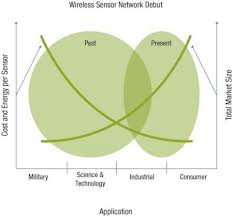
\includegraphics[scale=0.6]
		{figures/wsn_debut.jpeg}}
	\caption{\label{fig:my-label} Chuyển dịch thị phần của mạng cảm biến không dây}
\end{figure}

Đi liền với sự mở rộng việc ứng dụng mạng cảm biến không dây trong cuộc sống là các thách thức mới. Khi triển khai một mạng cảm biến trong thực tế, cần phải cân nhắc tới các tính chất, tính chất nào cần được ưu tiên hơn tính chất nào. Ví dụ với các địa hình khó xâm nhập như hang động, chiến trường, việc duy trì thời gian sống cho mạng cảm biến là yêu cầu thiết yếu, trong khi đó với các mạng để theo dõi như camera thì độ bao phủ là yếu tố hàng đầu. Việc lựa chọn giao thức, cách cài đặt, giao tiếp, đặt vị trí nhằm thu được một mạng cảm biến đáp ứng yêu cầu là một lĩnh vực nghiên cứu thu hút được nhiều sự quan tâm.

 
Chương đầu của đồ án đóng vai trò như cái nhìn tổng quan về mạng cảm biến không dây. Phần 1 sẽ bao gồm cấu tạo của một mạng cảm biến, các loại mạng khác nhau, giao thức mạng thường được sử dụng, các ứng dụng và khó khăn hiện thời khi triển khai mạng cảm biến không dây. Nhằm hỗ trợ cho việc giải thích chi tiết trong các chương sau, phần 1.2 sẽ là những kiến thức về khoa học máy tính nhằm giải quyết thách thức trong mạng cảm biến không dây được đề ra ở chương 2, cụ thể bao gồm: lý thuyết đồ thị và một số thuật toán sử dụng trên đồ thị, kiến thức về cấu trúc dữ liệu cây và bài toán cây Steiner để mô hình hóa bài toán mạng cảm biến không dây trong thực tế.

\section{Mạng cảm biến không dây}
\subsection{Định nghĩa và phân loại}
Mạng cảm biến không dây là một tập hợp các nút cảm biến tự động nhằm ghi lại dữ liệu của môi trường xung quanh, sau đó tổng hợp lại tại một trạm trung tâm để xử lý nhằm phục vụ cho mục đích giám sát, kiểm tra.\cite{koviwireless}


Có thể phân loại mạng cảm biến không dây thành các loại sau:
\begin{itemize}
\item Mạng cảm biến trên mặt đất: Mô hình mạng này bao gồm hàng trăm cho tới hàng ngàn nút cảm biến, triển khai rải rác trên mặt đất. Các vị trí đặt nút cảm biến có thể là trên chiến trường, trong rừng, trên núi. Có thể triển khai một cách tùy biến hoặc được lên kế hoạch từ trước, có thể sử dụng thiết bị bay để vận chuyển các nút cảm biến tới địa điểm mong muốn hoặc địa điểm con người khó tiếp cận.
\item Mạng cảm biến trong lòng đất: Mô hình này bao gồm các nút cảm biến được chôn sâu dưới lòng đất hoặc trong hang động, trong lòng núi nhằm đo đạc số liệu để dự báo thảm họa như núi lửa, động đất hay quan sát tình hình đất đai để có kế hoạch canh tác hợp lý. Vì trở ngại môi trường khó thay mới mà các nút cảm biến được lựa chọn cho địa hình này sẽ rẻ hơn so với loại triển khai trên mặt đất. 
\item Mạng cảm biến dưới nước: Mô hình này bao gồm các nút cảm biến thả dưới nước, có thể di chuyển được bằng bánh xe hoặc lực đẩy, liên lạc với nhau bằng sóng âm. Một ví dụ thực tế của mô hình này là Hệ thống giám sát âm thanh được nhắc tới ở phần đầu.
\item Mạng cảm biến truyền thông: Bao gồm các nút cảm biến thu dữ liệu truyền thông như camera, máy ghi âm. Bởi đặc tính của mạng truyền thông là kích thước gói tin lớn mà giao thức và đặc tính của các nút cảm biến cũng cần thay đổi để kết quả thu được không có độ trễ lớn. 
\item Mạng cảm biến di động: Các nút cảm biến trong mô hình mạng này có thể di chuyển để trao đổi thông tin hoặc sạc năng lượng. Khó khăn đặt ra trong mô hình này là tính toán độ bao phủ của mạng, giao thức truyền tin hợp lý, ít tiêu tốn năng lượng và chu trình sạc năng lượng của các nút cảm biến.
\end{itemize}
 
Hình 1.2 là hình ảnh trực quan về địa hình được triển khai và các nút cảm biến được cài đặt trong thực tế.


\begin{figure}[htb]
	\center{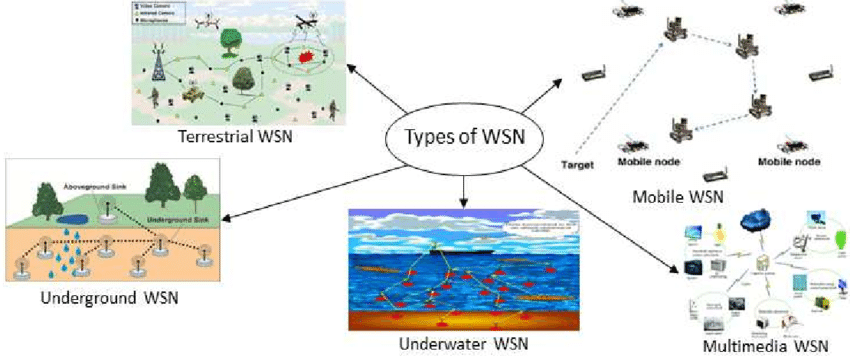
\includegraphics[width=\textwidth]
		{figures/wsn_types.png}}
	\caption{\label{fig:my-label} Các loại mạng cảm biến không dây}
\end{figure}

\subsection{Nút cảm biến}
Thành phần nhỏ nhất của một mạng cảm biến không dây là nút cảm biến. Cấu tạo của nút cảm biến bao gồm những bộ phận chính sau: bộ phận điều khiển, bộ phận chuyển tiếp, bộ nhớ, nguồn năng lượng, một hoặc nhiều bộ cảm ứng.
\begin{itemize}
\item Các thành phần cảm ứng là các thiết bị phần cứng, liên tục đo đạc những thông số của môi trường xung quanh, như là áp suất hay nhiệt độ, sau đó chuyển các tín hiệu liên tục này thành các tín hiệu số để xử lý tiếp bằng các thành phần khác. Có thể phân loại thành phần cảm ứng thành 3 loại: bị động - đa hướng, bị động - đơn hướng hoặc chủ động. Các thiết bị bị động - đa hướng chỉ ghi nhận dữ liệu mà không tác động trực tiếp với môi trường. Dữ liệu ghi nhận bởi thiết bị này không chỉ ra hướng thu nhận được, khác với các thiết bị bị động - đơn hướng như camera. Các thiết bị chủ động thì tác động tới môi trường, ví dụ bằng tia rada, và chúng cần được liên tục cấp năng lượng.
\item Bộ nhớ thì tùy thuộc vào yêu cầu mà được trang bị hay không. Vì mục tiêu tiết kiệm năng lượng mà bộ nhớ trên vi xử lý được ưu tiên hơn là bộ nhớ flash. Hai tác vụ chính của bộ nhớ bao gồm: lưu trữ dữ liệu và phục vụ cho tính toán.
\item Bộ phận xử lý có thể coi như là bộ não của nút cảm biến, chịu trách nhiệm thực thi nhiệm vụ, xử lý dữ liệu và điều khiển các bộ phận khác. Lựa chọn phổ biến là sử dụng vi điều khiển bởi tính tiết kiệm, tiêu thụ ít năng lượng và dễ dàng lập trình.
\item Bộ phận chuyển tiếp đóng vai trò cầu nối giữa các nút cảm biến, chịu trách nhiệm truyền và nhận các gói dữ liệu. Môi trường truyền tin sử dụng sóng radio, tia laze hoặc tia hồng ngoại. Tia laze thì sử dụng ít năng lượng, nhưng yêu cầu không gian truyền không được có vật cản. Tia hồng ngoại thì bị hạn chế bởi phạm vi giao tiếp. Bởi vậy phù hợp nhất với các ứng dụng của mạng cảm biến không dây là sử dụng sóng radio.
\end{itemize}
Vì thương được lắp đặt tại các vị trí khó tiếp cận, việc sạc hay thay pin dường như là không khả thi, bởi vậy mà nguồn năng lượng chính của các nút cảm biến thường sử dụng là pin. Tất cả các tác vụ bao gồm: cảm ứng, xử lý dữ liệu, chuyển tiếp dữ liệu đều tiêu tốn năng lượng, trong đó tốn kém nhất là dành cho việc truyền tin, bởi vậy việc duy trì sự sống của một nút hay giảm thiểu hóa việc sử dụng năng lượng luôn là một trong những tiêu chí phải cân nhắc khi triển khai một mạng cảm biến không dây.

Hình 1.3 là mô tả cấu trúc của một nút cảm biến trong mạng cảm biến không dây.


\begin{figure}[htb]
	\center{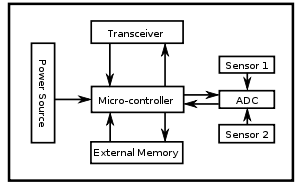
\includegraphics[width=\textwidth]
		{figures/sensor_node.png}}
	\caption{\label{fig:my-label} Cấu trúc một nút cảm biến}
\end{figure}

\subsection{Các giao thức truyền tin của mạng cảm biến}
Mạng cảm biến không dây có thể được triển khai bằng nhiều giao thức: \cite{akkaya2005survey}


\begin{itemize}
\item Dạng bus: Giao thức mạng đơn giản, được sử dụng khi có một số lượng ít nút cảm biến. Các nút thực hiện việc truyền tin qua hình thức quảng bá, tất cả các nút đều nhận được gói tin nhưng chỉ nút cảm biến đích là xử lý gói tin truyền tới. Tuy dễ dàng để cài đặt, giao thức dạng này cần phải có cơ chế xử lý xung đột hợp lý.
\item Dạng cây: Giao thức dạng cây được xây dựng theo cơ chế kế thừa, các nút con (là các nút cảm biến) có trách nhiệm đo đạc thông tin môi trường và truyền ngược lại các nút cha (có thể là các nút cảm biến hoặc chỉ là các nút truyền tin) để xử lý. Vì việc truyền và nhận tin thường tiêu tốn nhiều năng lượng nhất (so với việc xử lý hay lưu trữ), bởi vậy mà cần tìm đường truyền ngắn nhất đi từ nút con tới nút gốc.
\item Dạng hình sao: Giao thức này bao gồm một khu xử lý trung tâm nhận tất cả thông tin từ các nút xung quanh để xử lý. Tất cả việc giao tiếp đều phải thực hiện thông qua khu trung tâm này (giống với mô hình client - server). 
\item Dạng hình vòng: Các nút trong giao thức này được kết nối với chính xác 2 nút khác, việc truyền tin do đó được thực hiện tuần tự theo chiều kim đồng hồ hoặc ngược kim đồng hồ. Nếu có một nút bị chết thì toàn bộ mạng phải có cơ chế hồi phục lại.
\item Dạng hỗn tạp (Mesh Network): Giao thức mạng cho phép một nút có thể giao tiếp với các nút kề với nó, đồng thời có thể truyền tin theo nhiều hướng tới nút đích (khác với mạng hình vòng chỉ cho truyền theo 2 hướng).
\item Dạng kết nối đầy đủ (Fully connected Network): Giao thức mạng mà một nút kết nối với tất cả các nút khác trong mạng. Số lượng nút và số lượng kết nối giữa tất cả các nút tăng theo hàm lũy thừa khiến cho việc tính toán đường đi tối ưu cho gói tin rất khó khăn.
\end{itemize}
 
Hình 1.4 là tổng hợp của các giao thức thường được triển khai trong thực tế.


\begin{figure}[htb]
	\center{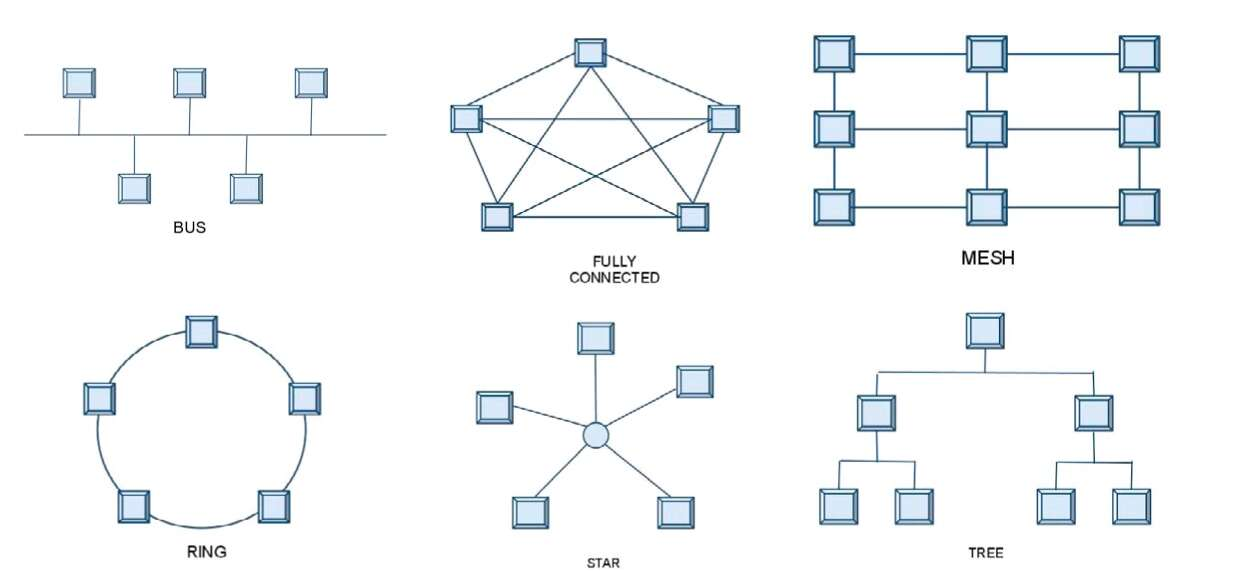
\includegraphics[width=\textwidth]
		{figures/wsn_topology.jpg}}
	\caption{\label{fig:my-label} Các giao thức mạng trong thực tế}
\end{figure}

\subsection{Ứng dụng của mạng cảm biến không dây}
Mạng cảm biến không dây từ những ngày đầu chỉ được ứng dụng trong quân sự và khoa học nay đã phát triển rộng rãi và cho thấy tác dụng lớn khi áp dụng vào trong những mặt khác của đời sống như: nông nghiệp, y tế, môi trường, xây dựng,v.v... Việc nhận thấy tiềm năng của mạng cảm biến không dây trong nhiều lĩnh vực của xã hội thúc đẩy khoa học và doanh nghiệp đẩy mạnh nghiên cứu, hợp tác để cho ra đời những nút cảm biến hiệu quả hơn, tiết kiệm hơn và các cơ chế triển khai mạng cảm biến tối ưu hơn. Dưới đây là bản nghiên cứu tác động của mạng cảm biến không dây trong các lĩnh vực khác nhau:\cite{ramson2017applications}
\begin{itemize}
\item Nông nghiệp: Các mạng cảm biến kết hợp của nhiều loại như dưới đất, trong lòng đất hay trong nước cung cấp thông tin cần thiết cho canh tác như nhiệt độ, độ ẩm, chất lượng đất, số lượng khí CO2 trong lòng đất, chất lượng nước,v.v... Dữ liệu được thu thập qua camera hoặc cảm biến, sau đó được xử lý và đưa tới chuyên gia để đưa ra quyết định sau cùng. Nhờ thông tin được truyền tải theo thời gian thực mà chuyên gia có thể phân tích tình trạng cây trồng, đất đai, nguồn nước để có cơ chế điều chỉnh thích hợp. Ngoài việc ghi nhận thông tin, các mạng cảm biến còn đóng vai trò tự động hóa quy trình canh tác, điều khiển để giảm thiểu công sức lao động, tăng năng suất và độ chính xác, giống như hệ thống thời gian thực được điều khiển bằng cảm biến tại các khu trồng trọt trong nhà kính.
\item Môi trường: Nhờ việc ghi nhận dữ liệu và truyền tải qua Internet mà có thể dự đoán trước các thiên tai tự nhiên như động đất, sóng thần, lũ lụt hay tai nạn lao động như rò rỉ khí ga, rò điện, qua đó giảm thiểu thiệt hại về người và của. Các ứng dụng thực tiễn trong môi trường có thể kể đến giám sát mức độ ô nhiễm môi trường, giám sát chất lượng nước và khí thải trong nhà máy, dự đoán nguy hiểm trong hầm mỏ như khí độc, nguồn lửa ngầm hoặc sập hầm. 
\item Giao thông: Giám sát giao thông là một ví dụ thực tiễn của mạng cảm biến truyền thông, kết hợp nhiều camera giám sát để thu được hình ảnh thời gian thực, hỗ trợ việc điều tiết, phân luồng, truy cứu trách nhiệm khi có tai nạn, xử lý vi phạm giao thông. Hệ thống giám sát giao thông đã được triển khai ở rất nhiều thành phố lớn trên thế giới giúp giảm thiểu lực lượng công quyền cần có mặt trực tiếp trên đường. 
\item Y tế: Các mạng cảm biến không dây được triển khai để giám sát sức khỏe của bệnh nhân, cụ thể là đo đạc thông số cơ thể như áp suất, chất béo, đặc biệt là ở người già, để có thể liên tục theo dõi và chăm sóc tình trạng. Bệnh nhân có thể đeo các thiết bị đo đạc và hệ thống sẽ tự động gửi thông tin về trung tâm liên tục để bác sĩ có thể chẩn đoán và đưa ra phác đồ điều trị một cách chính xác nhất.
\item Quân sự: Vai trò của mạng cảm biến không dây vẫn chưa hề mờ nhạt trong lĩnh vực quân sự, thậm chí là các mạng cảm biến hiện thời còn mang lại nhiều giá trị hơn. Giám sát kẻ địch, phát hiện xâm nhập, tính toán toán lộ trình là các mục tiêu chính khi triển khai mạng cảm biến không dây trên chiến trường.
\end{itemize}

\subsection{Khó khăn}
Như đã đề cập ở đầu chương, việc được ứng dụng rộng rãi ở nhiều lĩnh vực thúc đẩy những tiến bộ khoa học nhưng đồng thời cũng mang tới những thách thức khi triển khai một mạng cảm biến không dây trong thực tế. \cite{eisa2013challenges}


Một trong những thách thức lớn nhất và được ưu tiên hàng đầu khi thiết kế mạng cảm biến không dây là duy trì thời gian sống. Bởi đặc tính khó tiếp cận của môi trường đặt các nút cảm biến (trong lòng đất, trên chiến trường,v.v...) vậy nên việc sạc pin cho các mạng cảm biến hay đổi pin mới dường như là không thể. Hơn thế nữa với các giao thức mạng hình cây hoặc hình vòng, một nút chết trong mạng có thể dẫn tới việc tái định tuyến cho toàn bộ các nút khác. Từ hai nguyên do trên mà trước khi bắt đầu triển khai các nút cảm biến (có thể là chọn vị trí đặt hoặc xác định thuật toán định tuyến, giao thức truyền, giao thức xử lý xung đột), các kĩ sư đều phải lưu ý tới việc giảm thiểu năng lượng tiêu thụ. Nhưng bởi số lượng kênh hạn chế lại cần phải được chia sẻ giữa rất nhiều nút mạng, điều này có thể dẫn tới độ trễ lớn nếu quá ưu tiên vào việc bảo vệ năng lượng, khiến cho thông tin trở nên vô giá trị. Cân bằng giữa việc duy trì thời gian sống và đảm bảo hiệu quả trong giao tiếp là một bài toán khó, với những yêu cầu thay đổi tùy vào tình hình thực tế.


Ở những môi trường có khả năng xảy ra hư hại cho các nút cảm biến (chiến trường), một cơ chế chịu lỗi hay tái định tuyến là cần thiết để đảm bảo giao tiếp trong toàn mạng khi có vấn đề xảy ra. Ví dụ, một nút cần cập nhật lại bảng địa chỉ các mạng khác khi nhận thấy việc truyền tin như trước không hiệu quả. Cơ chế chịu lỗi cùng với cơ chế tự vận hành, khi các nút trong mạng đã được thiết lập thì có thể tự động thực hiện tác vụ mà không cần tới sự có mặt của con người, hỗ trợ cho tính tự động hóa của mạng cảm biến không dây, giảm thiểu chi phí lao động.
 

Đôi khi, các mạng cảm biến không dây cần được thiết kế để đảm bảo độ phủ trong truyền tin hay thông tin cần được truyền trong thời gian thực. Độ bao quát của mạng cảm biến phục vụ cho mục đích giám sát tổng quát như các lưới bảo vệ tại các cứ điểm quan trọng để phát hiện quân địch hay các khu vực rộng lớn như đất ruộng canh tác để thu thập đầy đủ dữ liệu. Trong khi đó đảm bảo chất lượng dịch vụ là một trong những yêu cầu của mạng truyền thông bởi con người rất nhạy cảm với độ trễ của âm thanh hay hình ảnh. Việc đảm bảo chất lượng đường truyền, chất lượng gói tin, trong khi vẫn duy trì thời gian sống của mạng là một thách thức không nhỏ.

\section{Lý thuyết đồ thị}
\subsection{Định nghĩa và biểu diễn đồ thị}
Đồ thị, trong phạm vi toán học, là một tập hợp những đối tượng được mã hóa thành các đỉnh và mối liên hệ giữa các đối tượng được mã hóa dưới dạng cạnh. (Hình 1.5 là một đồ thị đơn vô hướng)


\begin{figure}[htb]
	\center{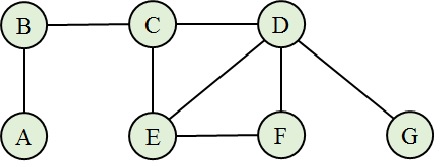
\includegraphics[width=\textwidth]
		{figures/undirected_graph.png}}
	\caption{\label{fig:my-label} Đồ thị đơn vô hướng}
\end{figure}
 
Đồ thị có thể được sử dụng để mô hình hóa rất nhiều bài toán trong thực tế: \cite{sedgewick2011algorithms}
\begin{itemize}
\item Bản đồ: Một bản đồ giữa các thành phố có thể là một đồ thị, trong đó các thành phố là các đỉnh, đường đi từ thành phố A tới thành phố B gần đó là một cạnh của đồ thị. Việc mô hình hóa như này có thể giúp giải các bài toán như xác định đường đi ngắn nhất từ một thành phố tới thành phố khác bằng các giải thuật trên đồ thị.
\item Internet: Các trang web trên mạng là các đỉnh của đồ thị và các hyperlink là các cạnh của đồ thị. Các thuật toán duyệt đồ thị đóng vai trò quan trọng trong các bộ công cụ tìm kiếm.
\item Lập lịch: Cơ chế lập lịch xuất hiện từ những nơi bé nhất như hệ điều hành cho tới nhà máy, sân bay. Việc lập một kế hoạch hợp lý, đáp ứng yêu cầu, đảm bảo một số ràng buộc như tài nguyên hay độ ưu tiên có thể được xử lý trước hết bằng cách mô hình hóa bằng đồ thị có hướng, sau đó áp dụng các thuật toán sắp xếp hoặc tìm kiếm đường đi trên đồ thị.
\end{itemize}
Tùy thuộc vào yêu cầu bài toán mà có thể lựa chọn mô hình đồ thị phù hợp, vô hướng hoặc có hướng, cạnh có trọng số hoặc không. Với đồ thị vô hướng, chiều cạnh nối 2 đỉnh là không quan trọng, có thể duyệt từ A tới B hoặc từ B tới A đều được, nếu tồn tại cạnh giữa 2 đỉnh A và B. Trong khi đó với đồ thị có hướng, giả sử hướng từ A tới B thì chỉ có thể duyệt từ A tới B. Chúng ta thường mô hình hướng của cạnh trong đồ thị bằng cách thêm dẫu mũi tên vào đích của cạnh, biểu thị chiều từ nguồn tới đích. Với trường hợp trọng số của cạnh, với các bài toán mà việc di chuyển từ đỉnh này tới đỉnh khác tiêu tốn tài nguyên (xăng dầu khi di chuyển trên đường, thời gian hoàn thành tác vụ,v.v...), các cạnh nối giữa 2 đỉnh sẽ được đánh trọng số thể hiện số tài nguyên sẽ tiêu tốn khi di chuyển trên cạnh này.
 

Cùng tùy thuộc vào yêu cầu của bài toán mà cách lưu trữ đồ thị trong bộ nhớ cũng khác nhau, nhưng có thể lựa chọn cách lai ghép để thu được hiệu quả từ cả 2. Cách lưu trữ sử dụng ma trận, mà phần tử a\begin{tiny}ij\end{tiny} là 0 hoặc 1 chỉ việc có tồn tại cạnh giữa 2 đỉnh i và j của đồ thị, sẽ tăng tốc việc truy cập nhưng lại tiêu tốn bộ nhớ. Trong khi đó nếu sử dụng các danh sách liên kết mà phần từ đầu là các đỉnh và các phẩn từ trong danh sách là các đỉnh liên kết với nó sẽ giúp giảm thiểu bộ nhớ sử dụng, nhưng tất nhiên việc truy xuất sẽ tiêu tốn thời gian hơn.

\subsection{Thuật toán duyệt đồ thị}
Duyệt đồ thị được hiểu là ghé thăm tất cả các đỉnh ở đồ thị (hoặc cho tới khi tìm được đỉnh cần thiết), mỗi đỉnh đúng một lần. Thuật toán duyệt đồ thị có thể được sử dụng như một cơ chế tiền xử lý cho các bài toán phức tạp khác như xác định chu trình hay tìm đường đi ngắn nhất.


Bên dưới là thuật toán Duyệt theo chiều rộng (Breadth-first search). BFS là quá trình thăm tất cả các đỉnh ở mức hiện tại (các nút kề với đỉnh đã xét gần nhất) trước khi thăm các đỉnh khác.


\begin{algorithm}
%\renewcommand{\thealgorithm}{}
\caption{Breadth-first search}\label{euclid}
\begin{algorithmic}[1]
\Procedure{BFS}{$Graph, Key$}
	\State Tạo hàng đợi rỗng
	\State Thêm nút gốc vào hàng đợi
	\State Tạo tập hợp các nút đã thăm
			
	\While {Hàng đợi vẫn chưa rỗng}
		\State nút $\leftarrow$ đầu hàng đợi
		\State Kiểm tra khóa của nút
		\State Thêm nút vào tập hợp đã thăm
		\State Thêm vào hàng đợi tất cả các đỉnh lân cận chưa được thăm của nút được xét gần nhất
	\EndWhile
\EndProcedure
\end{algorithmic}
\end{algorithm}


Thuật toán Duyệt theo chiều sâu (Depth-first search). DFS ngược lại so với BFS khi chúng ta ưu tiên thăm các đỉnh theo chiều sâu trước khi mở rộng ra các đỉnh lân cận.


\begin{algorithm}
%\renewcommand{\thealgorithm}{}
\caption{Depth-first search}\label{euclid}
\begin{algorithmic}[1]
\Procedure{DFS}{$Graph, Key$}
	\State Tạo stack rỗng 
	\State Thêm vào stack nút gốc
	\State Tạo tập hợp các nút đã thăm 
			
	\While {Stack vẫn chưa rỗng}
		\State nút $\leftarrow$ pop stack
		\State Kiểm tra khóa của nút
		\State Thêm vào stack tất cả các đỉnh lân cận chưa được thăm của đỉnh được xét gần nhất
	\EndWhile
\EndProcedure
\end{algorithmic}
\end{algorithm}

\subsection{Thuật toán xây dựng cây khung nhỏ nhất}
Cây khung nhỏ nhất là một đồ thị liên thông không có chu trình nối tất cả các đỉnh trong đồ thị. Hai thuật toán xây dựng cây khung nhỏ nhất được trình bày bên dưới là Kruskal và Prim.

 
\begin{algorithm}
%\renewcommand{\thealgorithm}{}
\caption{Kruskal's algorithm}\label{euclid}
\begin{algorithmic}[1]
\Procedure{Kruskal}{$Graph$}
	\State Create a forest where each vertex is a separate tree.
	\While {MST is not formed}
		\State Remove an edge from E with minimum weight
		\If {2 vertices belong to 2 different tree}
			\State Combine into a single one		
		\EndIf	
	\EndWhile 
\EndProcedure
\end{algorithmic}
\end{algorithm}

\begin{algorithm}
\renewcommand{\thealgorithm}{}
\caption{Prim's algorithm}\label{euclid}
\begin{algorithmic}[1]
\Procedure{Prim}{$Graph$}
	\State .
	\While {MST is not formed}
		\State Remove an edge from E with minimum weight
		\If {2 vertices belong to 2 different tree}
			\State Combine into a single one		
		\EndIf
	\EndWhile 
\EndProcedure
\end{algorithmic}
\end{algorithm}

\subsection{Lý thuyết về cây trong đồ thị}
Cây, trong mối liên quan với đồ thị, có thể được xem như một đồ thị liên thông, không có chu trình, trong đó ta chọn ra một đỉnh gọi là gốc. Hình ảnh trực quan là dễ dàng nhất để giúp định nghĩa những thành phần trong cây.
 

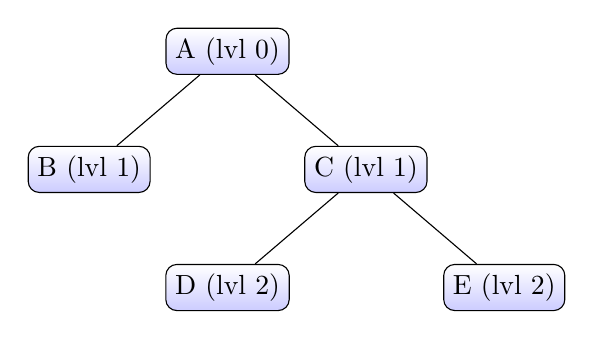
\begin{tikzpicture}[sibling distance=10em,
  every node/.style = {shape=rectangle, rounded corners,
    draw, align=center,
    top color=white, bottom color=blue!20}]]
 \node {A (lvl 0)}
    child { node {B (lvl 1)} }
    child { node {C (lvl 1)}
      child { node {D (lvl 2)} }
      child { node {E (lvl 2)} }
    };
\end{tikzpicture}


Fig 1.6


Các thành phần của một cây khi quan sát từ hình 1.6 bên trên sẽ bao gồm: nút A là nút gốc, nút B, C là các nút con của và tương ứng nút A là cha của chúng (nút C là cha của 2 nút D,E và D,E là con của C). (Vì chúng ta chỉ đề cập tới cây tổng quát nên sẽ không có khái niệm con trái hay con phải). Các nút D,E được gọi là các nút lá nếu không có bất kỳ con nào. Một cây có nhiều mức, các cây cùng một cha sẽ cùng một mức (hoặc có cha cùng mức thì cũng có cùng mức) và sẽ có mức lớn hơn mức cha là 1. Bắt đầu từ nút gốc có mức 0, các nút B,C sẽ có mức 1, D,E có mức 2. Chiều cao của cây là đường dài nhất đi từ gốc tới nút lá bất kỳ, hay được tính đơn giản bằng mức sâu nhất.

\subsubsection{Cây Steiner}
Trong phạm vi tổng quát, cây Steiner là một tập các bài toán trong lĩnh vực tổi ưu hóa tổ hợp. Nhưng để tập trung vào vấn đề tiếp theo sẽ giải quyết ở chương 2, chúng ta chỉ quan tâm tới cây Steiner trong đồ thị, có thể được diễn giải một cách đơn giản như sau: một cây Steiner là một cây có trọng số nhỏ nhất chứa tất cả những đỉnh cần thiết (là một tập con của tất cả các đỉnh trong đồ thị), cây có thể bao gồm các đỉnh khác hoặc không. Khái niệm trọng số nhỏ nhất ở đây có thể hiểu là tối thiểu hóa hàm mục tiêu (các mục tiêu có thể là thời gian sống trong mạng, độ bao phủ của các nút cảm biến, độ trễ của đường truyền, v.v...) đối với các bài toán trong mạng cảm biến không dây. Khi số lượng nút Steiner (các nút bắt buộc xuất hiện trong cây) bằng với số nút trong đồ thị, ta có thể quy về bài toán cây khung nhỏ nhất. Còn khi chỉ có 2 nút Steiner thì ta có thể quy về bài toán đường đi ngắn nhất. Mặc dù vậy, tuy 2 bài toán trên có thể giải trong thời gian đa thức, cây Steiner lại thuộc lớp NP-complete.\cite{karp1972reducibility}

\section{Tổng kết}
Chương 1 bao gồm những kiến thức tổng quan về lĩnh vực mà đồ án nghiên cứu (mạng cảm biến không dây), và một số phạm trù khoa học máy tính liên quan tới bài toán đặt ra (đồ thị và cây Steiner). Cụ thể, phần 1.1 cho biết những giao thức mạng thường được sử dụng, ứng dụng và khó khăn khi triển khai một mạng cảm biến không dây trong thực tế. Kiến thức trong phần này có thể giúp những người mới tiếp cận dễ dàng hơn với một trong những lĩnh vực đang thu hút nhiều sự quan tâm của giới nghiên cứu cũng như có cái nhìn bao quát về sự hiện diện của mạng cảm biến không dây trong đời sống. Phần 1.2 đóng vai trò như sự bổ sung kiến thức cho phần diễn giải chi tiết ở chương sau, đặc biệt là phần giải mã của các thuật toán sẽ được áp dụng đã được trình bày chi tiết, cụ thể là thuật toán BFS để duyệt cây và Kruskal để xây dựng cây con nhỏ nhất.